\documentclass[slidestop,red]{beamer}
\usepackage{beamerthemesplit}
\usepackage{polski}
\usepackage[utf8]{inputenc}

\usepackage{color}
\usepackage{listings}
\lstset{language=Python,
    basicstyle=\ttfamily\bfseries,
    commentstyle=\color{red}\itshape,
  stringstyle=\color{darkgreen},
  showstringspaces=false,
  keywordstyle=\color{blue}\bfseries}

\mode<presentation>{
   \setbeamertemplate{background canvas}[vertical shading][bottom=red!10,top=blue!10]
      \usetheme{Darmstadt}
      \usefonttheme[onlysmall]{structurebold}
	 }


% TikZ
\usepackage{tikz}
\usetikzlibrary{arrows}
\tikzstyle{block}=[draw opacity=0.7,line width=1cm]


\usepackage{geometry}
\usepackage{hyperref}


\def\hilite<#1>{
\temporal<#1>{\color{gray}}{\color{blue}}{\color{black}}
}


\title{Tytuł Twojej pracy dyplomowej}
\author{Twoje imię i nazwisko}
\date{\today}

\usepackage[pages=some,scale=1,angle=0,opacity=0.7]{background}

\begin{document}
\logo{\put(-365,0){
\includegraphics[scale=0.2]{logo_copernicus.png}}}
\frame{\titlepage}


\section{Projekt systemu}

\subsection{Założenia}
\frame
{
	\begin{block}{}
		\begin{itemize}
                    \item Wylistowany tekst
					\item Wylistowany tekst
                    \item Wylistowany tekst
					\item Wylistowany tekst
					\item Wylistowany tekst
					\item Wylistowany tekst
					\item Tekst
        \end{itemize}
        \end{block}

}
\subsection{Implementacja}
\frame
{
	\begin{block}{}
		\begin{itemize}
                    \item Wylistowany tekst
					\item Wylistowany tekst
                \end{itemize}
                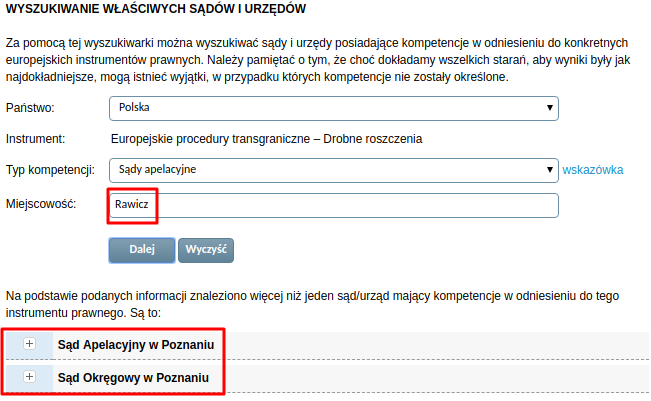
\includegraphics[scale=0.4]{rawicz.png}
        \end{block}
}
\subsection{Implementacja}
\subsubsection{Dane wejściowe}
\frame
{
	\begin{block}{}
		\begin{itemize}
                    \item Wylistowany tekst
                \end{itemize}
                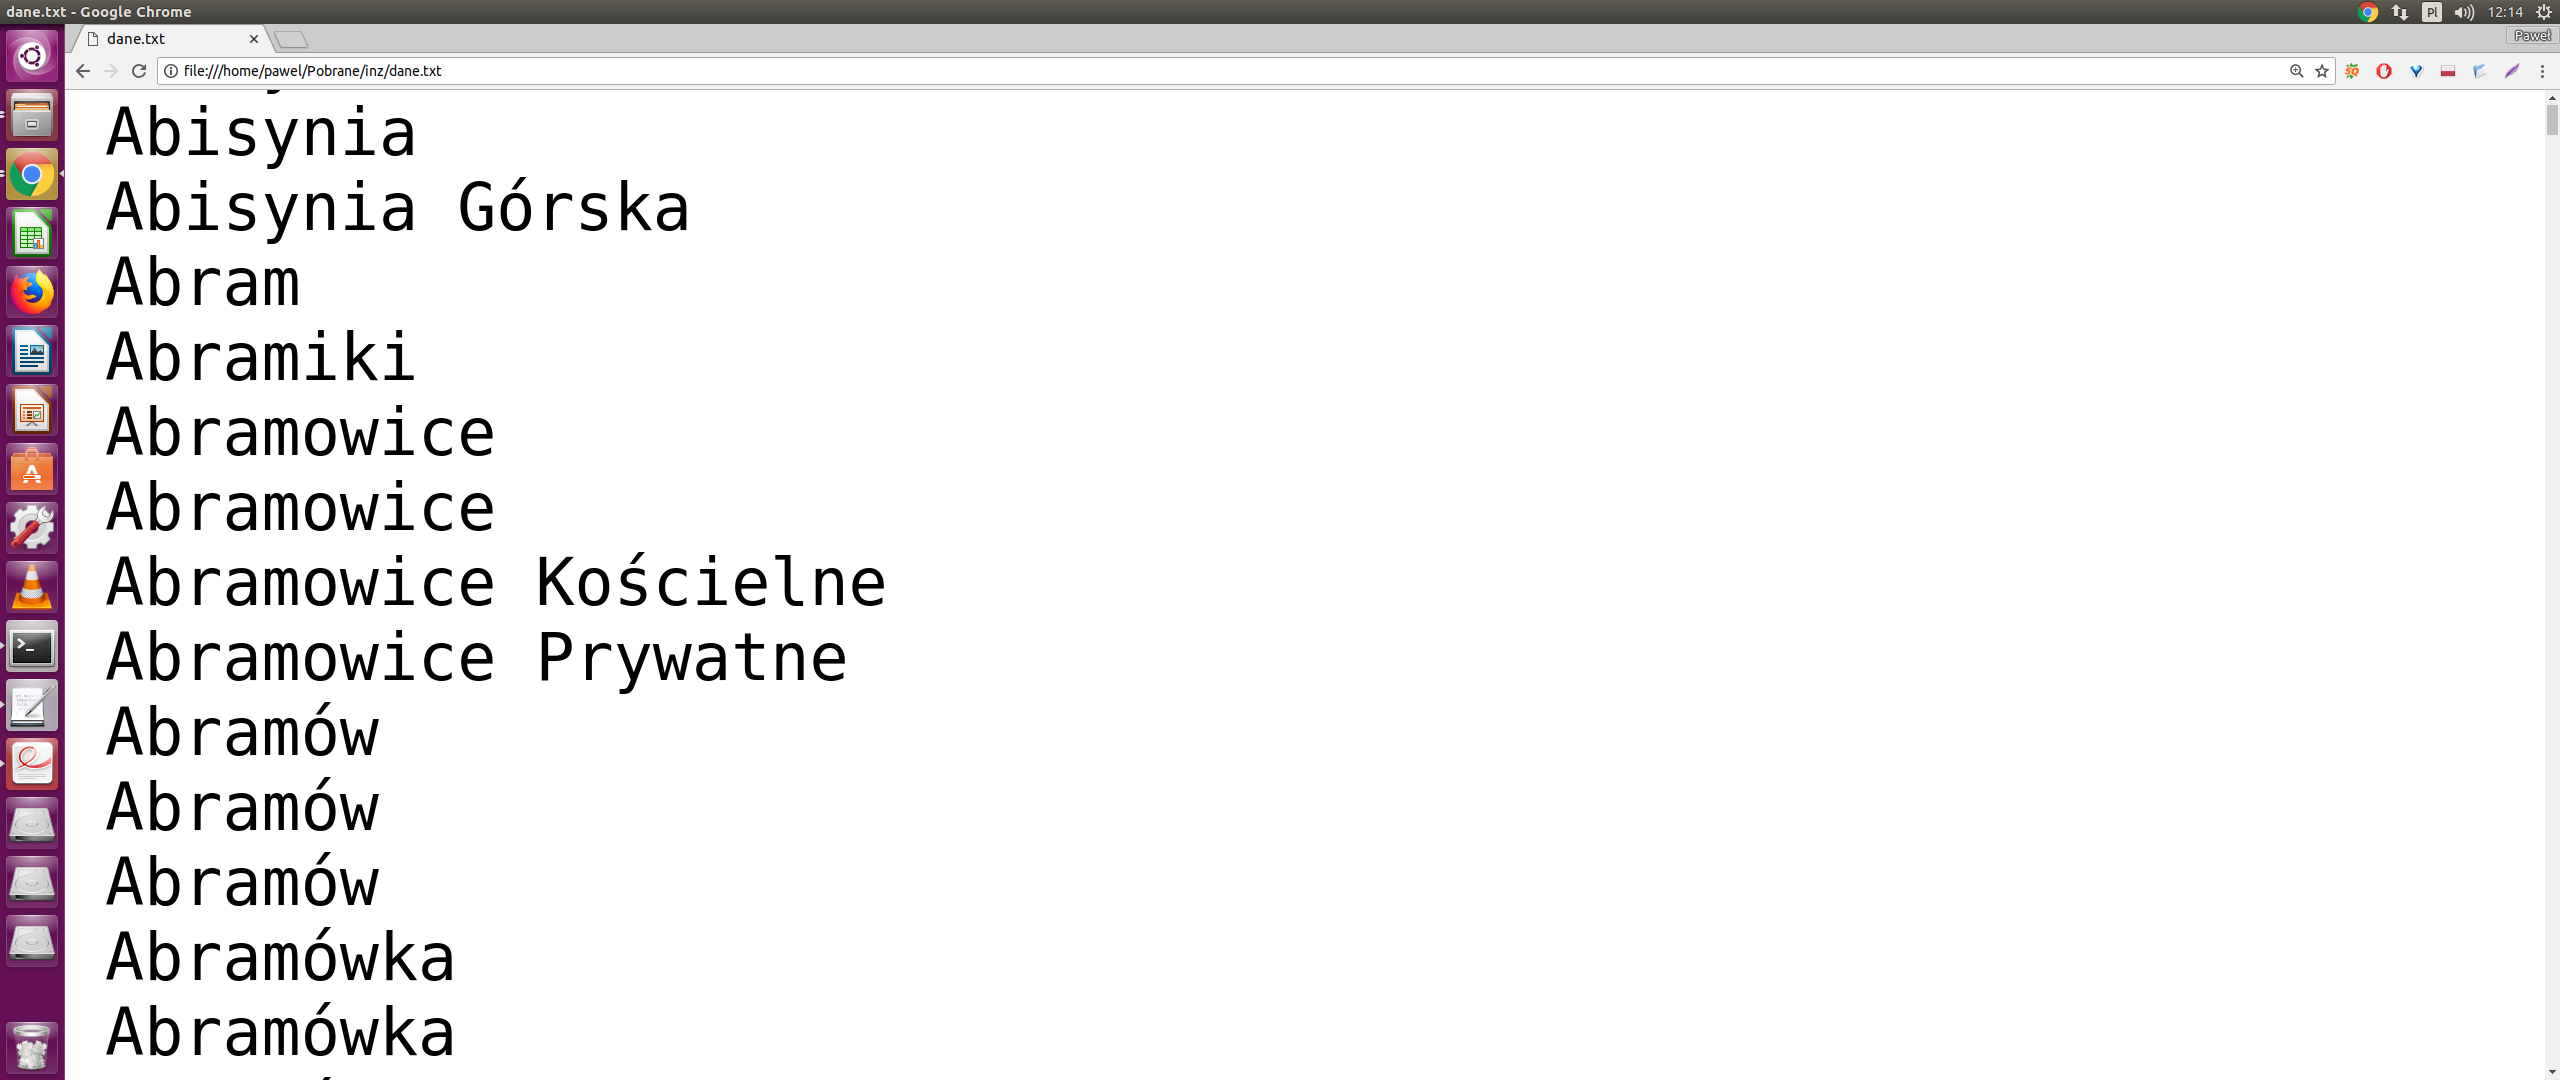
\includegraphics[scale=0.12]{dane-wejsciowe.png}
        \end{block}
}
\subsection{Implementacja}
\subsubsection{Dane wejściowe}
\frame
{
	\begin{block}{}
		\begin{itemize}
                    \item Wylistowany tekst
                \end{itemize}
                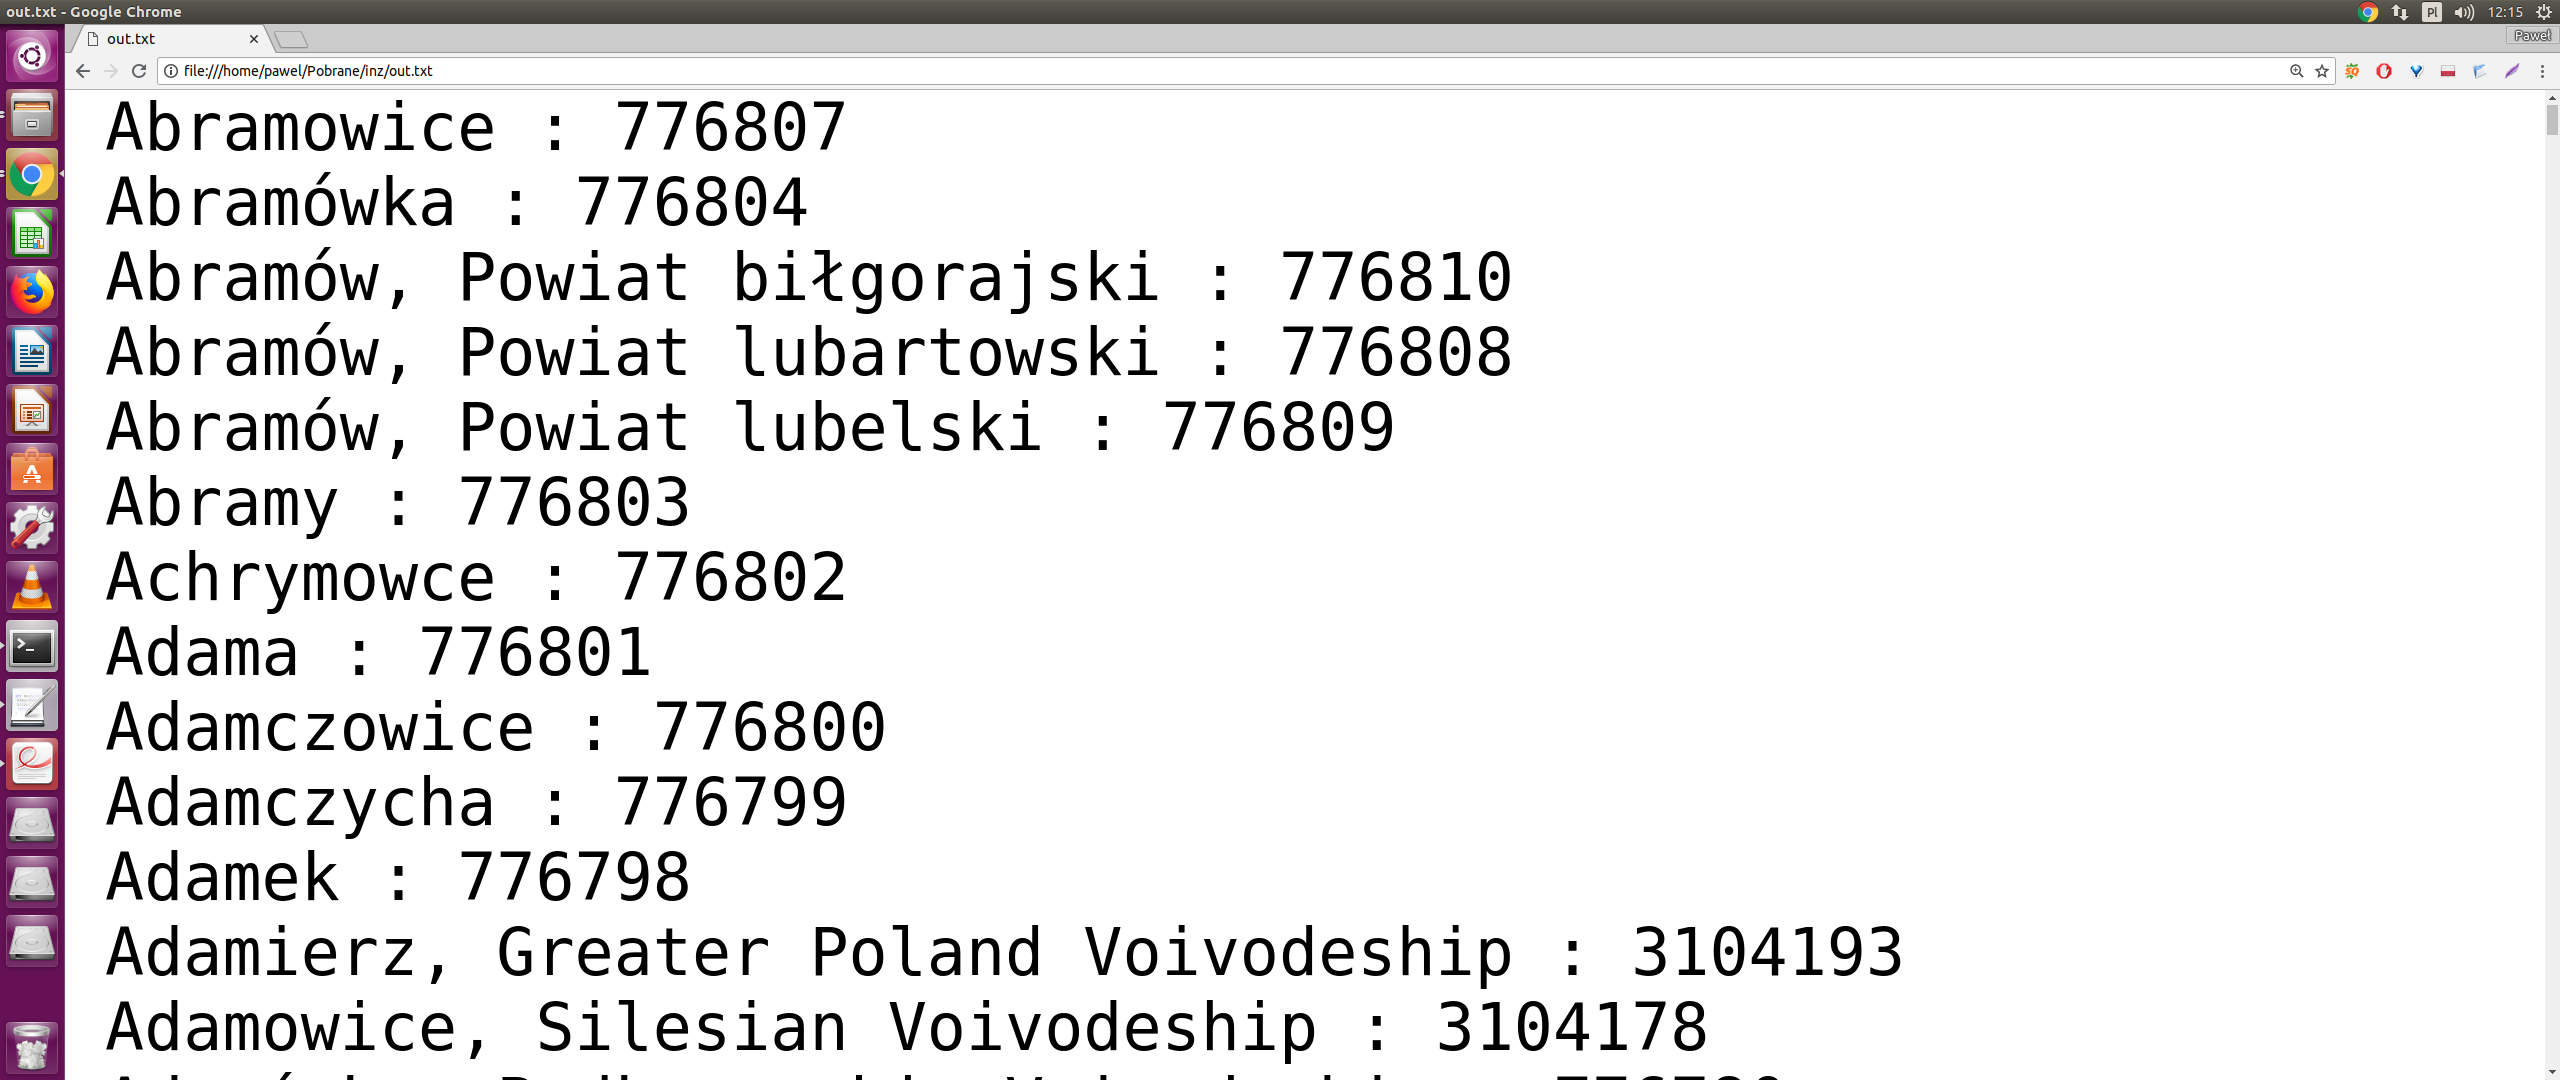
\includegraphics[scale=0.12]{dane-wyjsciowe.png}
        \end{block}
}

\subsection{Pozostało do zrobienia}
\frame
{
	\begin{block}{}
		\begin{itemize}
                    \item Wylistowany tekst
                \end{itemize}
                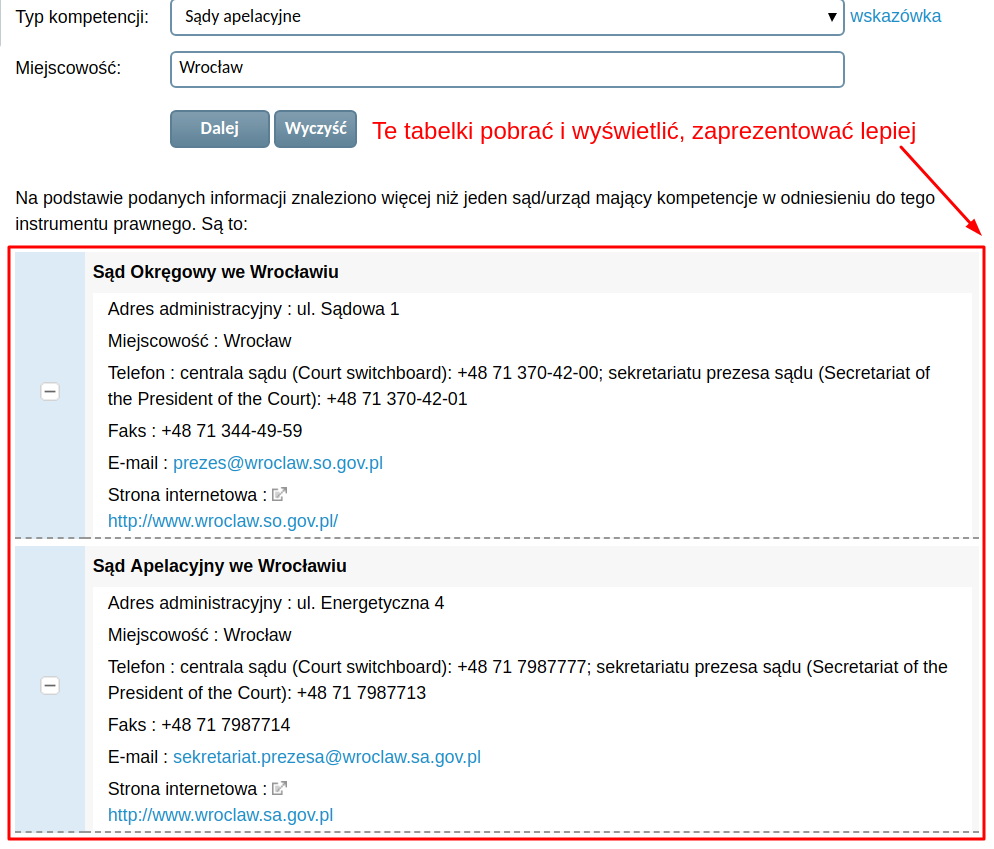
\includegraphics[scale=0.22]{to-wyswietlic.png}
        \end{block}
}

\subsection{Zakończenie}
\frame
{
\begin{center}
\begin{block}{}
        \centering Dziękuję za uwagę
\end{block}
\end{center}
}
\end{document}
